
                \begin{figure}
                    \centering
                    \begin{tikzpicture}
                        \pgfplotsset{%
                            width=1\textwidth,
                            height=0.4\textheight
                        }
                        \begin{axis}[
                            xlabel={Runs since restart},
                            ylabel={Average dynamic energy (watt)},
                            ymin=0,ymax=70,
                        ]
                        
                            \addplot [mark=none, densely dashed, red]  coordinates {
                            (1, 0.028600939828388666)(2, 0.006392984923953349)(3, 0.0012750723053127078)(4, 0.0010212833518232767)(5, 0.0008710893006795098)
                            };
                            \addlegendentry{workstation - IntelPowerGadget}
                            
                            \addplot [mark=none, densely dashed, blue]  coordinates {
                            (1, 0.008422471455823866)(2, 0.004229054025317184)(3, 0.0028731276234540784)(4, 0.0012553261023506475)(5, 0.0010040373736633172)
                            };
                            \addlegendentry{workstation - HardwareMonitor}
                            
                            \addplot [mark=none, densely dashed, cyan]  coordinates {
                            (1, 0.0)(2, 0.0)(3, 0.0)(4, 0.0)(5, 0.0)
                            };
                            \addlegendentry{workstation - Clamp (win)}
                            
                        \end{axis}
                    \end{tikzpicture} 
                \caption{A graph illustrating the energy consumption of Dram for test case Nbody with regards to how long ago the DUT was restarted, experiment \#2, (without outliers)} \label{fig:Nbody_Dram_iteration_exp2}
                \end{figure}
                